\begin{flushleft}
Per testare le precedenti funzioni abbiamo implementato il seguente script:
\lstinputlisting[language=Matlab]{cap_5/es5/es5.m}
Il sistema $Ax=b$ è formato dagli elementi:
\[
A = \left(\begin{array}{ccc} -4 & 2 & 1\\ 1 & 6 & 2\\ 1 & -2 & 5 \end{array}\right)
\]
\[
b = \left(\begin{array}{c} 1\\ 2\\ 3 \end{array}\right)
\]
Partendo dal vettore iniziale:
\[
x_0 = \left(\begin{array}{c} 0\\ 0\\ 0 \end{array}\right)
\]
Come possiamo vedere dall'output:
\begin{figure}[H]
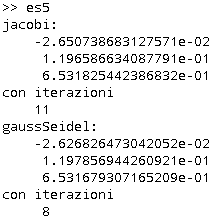
\includegraphics[left, width=350px, height=150px]{cap_5/es5/es55.png}
\end{figure}
Le nostre function restituiscono in output il vettore risultato e il numero di iterazioni che ha svolto.
\end{flushleft}